% Flowchart
% Author: Stefan Kottwitz
% https://www.packtpub.com/hardware-and-creative/latex-cookbook
%\documentclass{standalone}
\documentclass{standalone}
%\usepackage{geometry}
\usepackage{tikz}
\usetikzlibrary{matrix,calc,shapes}
\tikzset{
treenode/.style = {shape=rectangle, rounded corners,
                   draw, anchor=center,
                    text width=6em, align=center,
                    top color=white, bottom color=blue!20,
                    inner sep=1ex},
decision/.style = {treenode, diamond, inner sep=0pt},
root/.style     = {treenode, font=\Large, bottom color=red!30},
env/.style      = {treenode, font=\ttfamily\normalsize},
finish/.style   = {root, bottom color=green!40},
dummy/.style    = {circle,draw}
}

\newcommand{\yes}{edge node [above] {yes}}
\newcommand{\no}{edge  node [left]  {no}}

\begin{document}
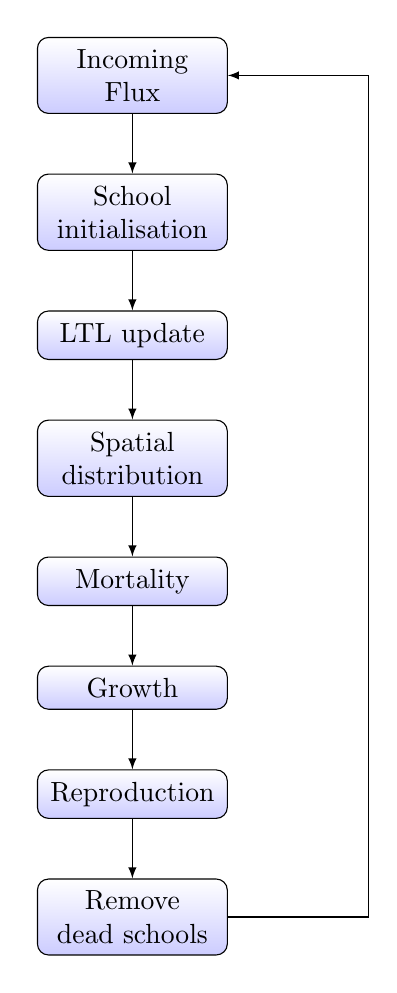
\begin{tikzpicture}[-latex]
\matrix (chart)
[
matrix of nodes,
column sep      = 3em,
row sep         = 5ex,
column 1/.style = {nodes={treenode}},
column 2/.style = {nodes={treenode}}
]
{
    Incoming Flux\\
    School initialisation \\
    LTL update \\
    Spatial distribution\\
    Mortality\\
    Growth\\
    Reproduction \\
    Remove dead schools \\
};

\draw (chart-1-1) edge (chart-2-1)
\foreach \x/\y in {2/3, 3/4, 4/5, 5/6, 6/7, 7/8} {
    (chart-\x-1) edge (chart-\y-1)
};
\draw (chart-8-1) -- +(3, 0) |- (chart-1-1);

%\foreach \x in {2,...,6} {
%(chart-\x-1) \yes (chart-\x-2) }
%(chart-7-3) \no  (chart-8-3)
%(chart-8-3) edge (chart-8-4);

%\draw
%(chart-6-1) -- +(-2,0) |- (chart-1-1)
%node[near start,sloped,above] {no, reconsider};
%\foreach \x in {2,...,6} {
%\draw   (chart-7-3)  -| (chart-8-4)
%node[near start,above] {yes}; 
\end{tikzpicture}
\end{document}

